\section{Matching and Inference}
\label{sec:match_inf}

\textit{Matching} formulas in semantically parsed stories to formulas in schemas underlies both learning and inference. The formulas comprising a schema are intended to be relatively simple---with complex conjunctions split into separate formulas---and unifiable with formulas parsed from real stories. Unification of a story formula with a schema formula binds individual constants from the former to variables in the latter. These bindings are then substituted in the rest of the schema instance, thereby ``filling in'' some of the missing information. %% I thought the following caveat is needed. -LS
This information is likely to be correct if the story events and participant types matched to the schema can be assumed to provide good evidence for an occurrence of the stereotyped pattern of events the schema captures, i.e., if the schema can be considered to have been ``confirmed'' by the observations.
We refer to any schema instance with one or more bound variables as a \textit{match}.

\begin{figure}
    \centering
    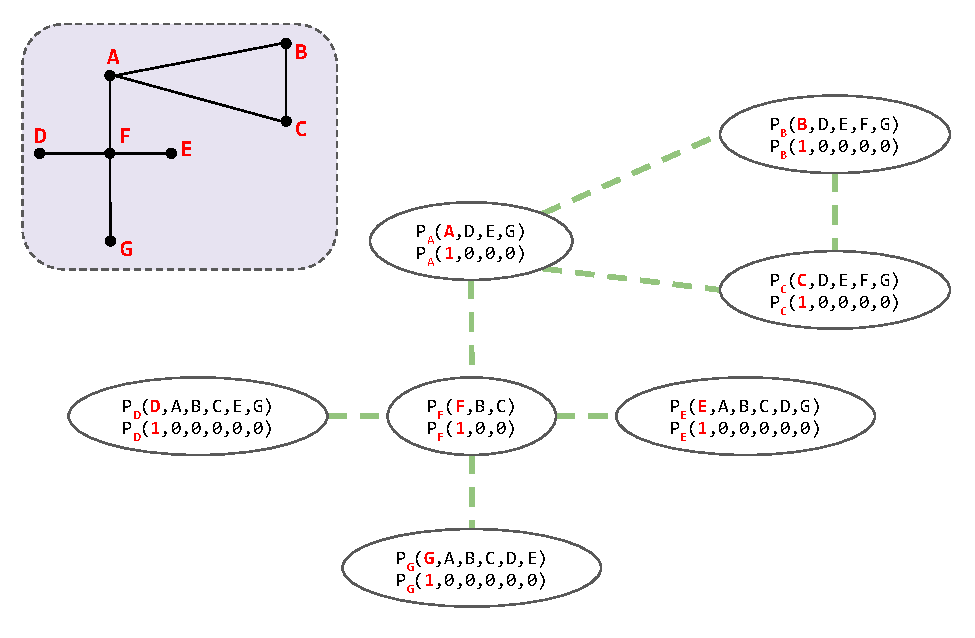
\includegraphics[width=0.75\columnwidth]{CH3_schemas/match_clique_reduction.pdf}
    \caption{A transformation of an example graph input for the weighted maximum clique problem (upper left) into EL propositional input for the schema matching problem. The green dotted lines in the latter input denote non-contradictory pairs of variable bindings. This transformation is used in the $\mathrm{NP}$-hardness proof for schema matching given for Theorem~\ref{thm:npcomplete}.}
    \label{fig:match_transformation}
\end{figure}

More formally, given a set of story ELFs $\Phi$ and a set of schema formulas $\Psi$, we define a match as a set of edges between elements of $\Phi$ and $\Psi$ such that no element of either touches more than one edge. These edges represent EL formula unification operations $\sigma(\phi, \psi) = (b_{\phi,\psi}, s_{\phi,\psi})$, where $b_{\phi,\psi}$ is the variable binding function produced by the unification, and $s_{\phi,\psi}$ is the score of the unification. Another constraint exists on valid matches: each variable $v$ in the schema must be bound to at most one unique value across \textit{all} variable binding functions $b_{\phi,\psi}$ for all unifications. We show that the problem of selecting a valid set of unification edges $E \subset \Phi \times \Psi$ with maximal weight $\sum_{(\phi,\psi) \in E} s_{\phi,\psi}$ is $\mathrm{NP}$-hard with the following reduction from the weighted maximum clique (WMC) problem:

\newtheorem{theorem}{Theorem}
\begin{theorem}
\label{thm:npcomplete}
Optimal story-schema matching is $\mathrm{NP}$-hard.
\end{theorem}
\begin{proof}
Let the graph input to the WMC problem be $G = (V={v_{0}, v_{1}, ..., v_{|V|}},E)$ with weight function $w : V \to \mathbb{R}$.

For each vertex $v_{i}$, we construct a pair of EL propositions $\phi_{i} = \text{P}_{i}(1,0,0,...)$ and $\psi_{i} = \text{P}_{i}(v_{i},v_{a},v_{b},...)$ where $v_{a},v_{b},...$ is a sequence containing all vertices \textit{not} sharing an edge with $v_{i}$, each of which is aligned with a $0$ in the corresponding proposition.
$\phi_{i}$ and $\psi_{i}$ can respectively be called the \textit{story} and \textit{schema} propositions.
An illustrated example of this transformation is shown in Figure~\ref{fig:match_transformation}.

Because the predicate $P_{i}$ for both propositions is the same, and unique to $v_{i}$, each of the two propositions may only unify with the other, or with nothing.

We also define the EL unification score function to be $s_{\phi_{i},\psi_{i}} = w(v_{i})$.

An optimal solution to the schema matching problem with these propositions as input will include only proposition unification pairs whose values for all bound variables are mutually compatible.

Because the pair of propositions corresponding to each vertex assigns the value $1$ to its own vertex's variable, and all unconnected vertices are assigned the contradictory value $0$, no two proposition unifications for unconnected vertices may co-exist in any solution, meaning the solution will correspond to a clique.

And because the solution will have maximal score, it will correspond to the clique with maximal weight in the original graph.
\end{proof}

Because the schema matching problem is $\mathrm{NP}$-hard, we need an efficient approximation for practical use. For our schema inference experiment (Section~\ref{sec:inf_eval}), we implement a basic matching algorithm that operates given an EL parse of a story and a pre-selected candidate schema (Algorithm~\ref{alg:matching}). The algorithm reduces the space of possible alignments and then samples the space several times, returning the best found solution. The simplicity of that algorithm is due to the limited scale of the experiment. Schema candidate selection becomes difficult as the corpus of learned schemas grows large, but with only dozens of learned schemas at this stage in the project, our corpus is not yet large enough to perform meaningful experiments with large-scale candidate selection. Similarly, the schemas learned so far have been individually quite simple, with at most one nesting level and a handful of formulas each. Our current matching algorithm is only intended to deal with matching stories to schemas of that scale, and as such will likely require substantial refinement as learned schemas grow in complexity. The basic matching algorithm was also developed using only a small development corpus of three learned schemas, resulting in largely intuited heuristics, such as its scoring function, that have yet to be tested at scale. Nevertheless, we include here a description of the basic schema matching algorithm used in our inference experiments.

\subsection{Basic Matching Algorithm}
\label{sec:basic_algo}

Using EL formula unification as a primitive, we implemented basic schema matching (Algorithm~\ref{alg:matching}) by iterating through the formulas in an EL parse of a story, matching each formula to any schema formula retrieved as a candidate, and applying the bindings to the schema. When the story has been fully iterated through, or all schema variables have been bound, the match is complete.
Algorithm~\ref{alg:matching} does not account for nested schemas; nested schemas can be ``flattened'', however, with all of their formulas placed inside the nesting schema, to allow the matching algorithm to match at all nesting levels without modification.
Because the order of formula matches can affect what variables are bound, and therefore which formulas may be subsequently matched, we randomly permute story formulas and unify them, in the randomized order, with schema formulas.
We try multiple permutations to explore the space of possible matches, searching for the highest scoring match, and cache low-level unification results to speed up the process.
We minimize the number of unification attempts by first unifying all story individuals and schema variables with shared types, provided they are each the only individual with that type in their source.
When shuffling the story formulas, we also independently shuffle the episodic formulas and the non-episodic formulas, thereafter placing the shuffled episodic formulas ahead of the others; this is because fluent schema formulas often bind many variables while having relatively few candidate matches.

\begin{algorithm}
\caption{A basic algorithm for matching a story to a schema.}
\label{alg:matching}
\begin{algorithmic}
\STATE INPUT: set of story EL formulas $STORY$, a candidate schema $SCH$, number of shuffles $SHUF$, match scoring function $score$
\STATE OUTPUT: best schema $match$
\STATE $match \gets null$
\STATE $SCH \gets flatten(SCH)$
\STATE $B_{cur}$ are empty bindings
\FOR{$V$ in $variables(SCH)$}
    \FOR{$I$ in $individuals(STORY)$}
        \IF{$type(V) = type(I)$ and no other variables/individuals have the same type}
            \STATE bindings $B_{cur}$ are updated to bind $V$ to $I$
        \ENDIF
    \ENDFOR
\ENDFOR
\FOR{i from 0 to $SHUF$}
    \STATE $STORY \gets shuffle(STORY)$
    \FOR{$\phi$ in $STORY$}
        \FOR{$\psi$ in $SCH$}
            \IF{$\phi$ and $\psi$ unify under bindings $B_{cur}$ to make variable bindings $B_{new}$}
                \STATE $B_{cur} \gets \text{all new bindings in} \  B_{new}$
            \ENDIF
        \ENDFOR
    \ENDFOR
    \IF{$score(SCH) > score(match)$}
        \STATE $match \gets SCH$
    \ENDIF
\ENDFOR
\end{algorithmic}
\end{algorithm}

\subsubsection{Scoring}
\label{sec:scoring}
When a schema is matched to a story, some constraints may be broken; this is a natural part of the learning process. A schema for a cow eating grass matched to a story about a dog eating grass violates the cow constraint on a participating entity, but is a valuable source of knowledge if properly generalized. On the other hand, too many broken constraints are indicative of a poor match between a schema candidate and a story.
Schema matches are heuristically scored by counting satisfied constraints, weighted by constraint type.
Confirmed role constraints are worth half as many points as confirmed step events.
Confirming the schema's header formula is worth twice the points of any other event.
For inexact matches---e.g., \texttt{(?X COW.N)} and \texttt{(ROVER.NAME DOG.N)}---the score of the binding is further weighted by the approximate semantic similarity of the two words. If one subsumes the other in the WordNet hypernym hierarchy, the strength is scaled by the distance of the two in that hierarchy. If neither subsumes the other, but they share a common ancestor hypernym, the strength is half their average distance to that ancestor.
The hypernym score accounts for half of the overall weight of an inexact match; the other half is provided by their semantic similarity according to a pre-trained word embedding model.\footnote{\textit{GoogleNews-vectors-negative300.bin}, \citet{NIPS2013_5021}}

We evaluate the quality of a partial schema match in terms of the number of formulas in the schema that are present in the observed story after making appropriate variable substitutions. However, schemas would not be useful for inference if we required all of its formulas to be matched to observations; their inferential capacity is a result of their expected \textit{over}-coverage of typical stories instantiating them. When the highest-scoring match of a story to a schema has been obtained, we must decide whether to \textit{abandon} the match due to its unsuitability for the story; or whether, instead, to \textit{confirm} the match, treating its unmatched formulas as (at least tentative) inferences. Identifying which subsets of matched formulas \textit{suffice} to imply the truth of which subsets of unmatched formulas is itself a complicated problem with a large combinatorial space. Because the inference experiment in Section~\ref{sec:inf_eval} begins with stories known to match the schemas being evaluated, this matching algorithm does not currently make such determinations. The construction of an effective heuristic for doing so would likely require a larger and more diverse corpus of schemas than we have been able to learn and assess as of this writing.